\documentclass[12pt]{article}
\usepackage[a4paper, bindingoffset=0.2in, %
							left=0.5in,right=0.5in,top=0.5in,bottom=0.5in,%
							footskip=.25in]{geometry}
\usepackage{graphicx}
\usepackage{listings}
\usepackage{amssymb}
\usepackage{amsmath}
\usepackage{hyperref}


\title{PSet3 Report}
\author{Ali Abolhassanzadeh Mahani}
%\date{Oct. 15}

\begin{document}
	\maketitle
	
	\section{Coloring Algorithm}
	I added a new vertical array to the left side of my grid to initialize the clusters. The algorithm is as you said
	in your class. I used numbers from 1 to ... for the cells that are \emph{on} and 0 for cells that are \emph{off}.
	Now you can see the picture in Fig \ref{fig:Color}
	\begin{figure}[h!]
		\centering
		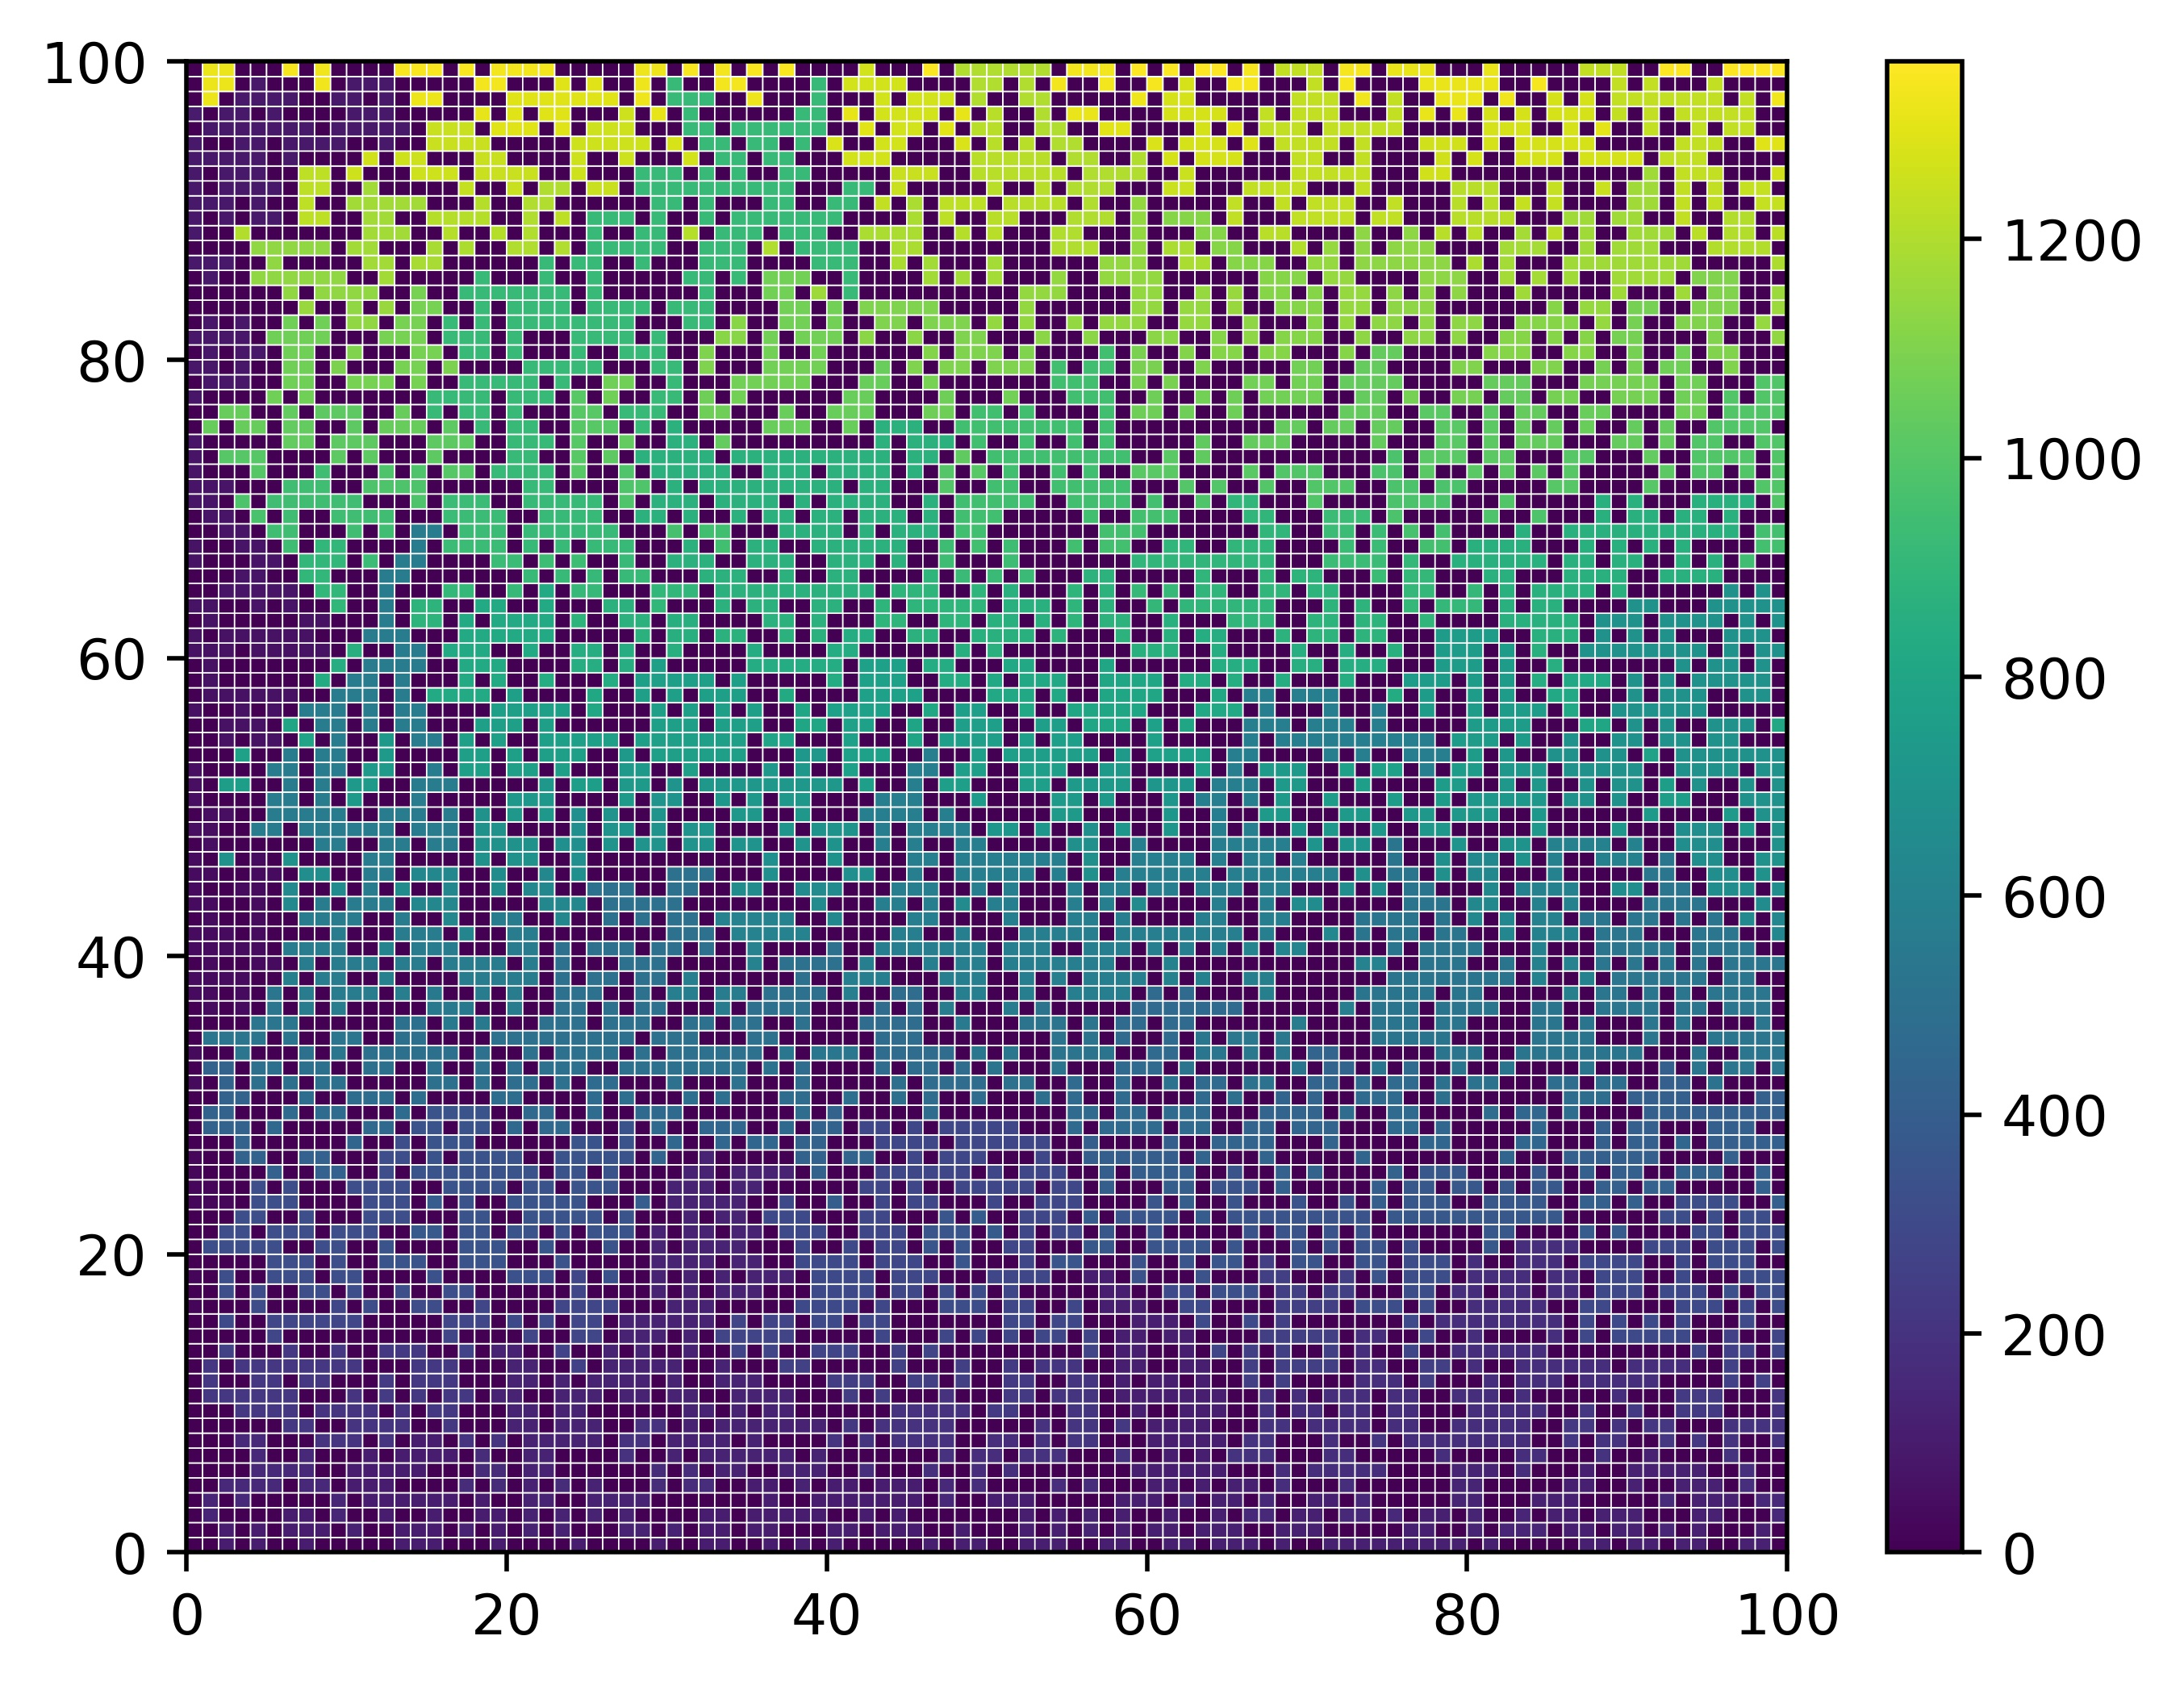
\includegraphics[width=0.9\linewidth]{../p2/colored.jpg}
		\label{fig:Color}
		\caption{Simulation of horizontal percolation for a 50 * 50 grid with probability 0.5. The cells with number 0 are \emph{off} and the ones with the same color form a \emph{clutser}}
	\end{figure}
\end{document}